\section{Corn}

Corn or Maize (\textit{Zea mays L.}) is a grain crop that yields large kernels set in rows on a cob. It is highly important in the agriculture sector in many countries around the world. Developed countries consume corn as a second-cycle product (e.g. in the form of meat, eggs and dairy products) while on developing countries, it is consumed directly. This crop serves as a staple diet for some 200 million people. Furthermore, this crop does not only serve as food; it can be processed into another form such as fuel (ethanol) and starch for other purposes. The many varieties of corn yield numerous products both for human and livestock consumption.~\cite{Jean2003} Figure \ref{fig:corn} shows a picture of Maize.

\begin{figure}[!htbp]
	\centering
		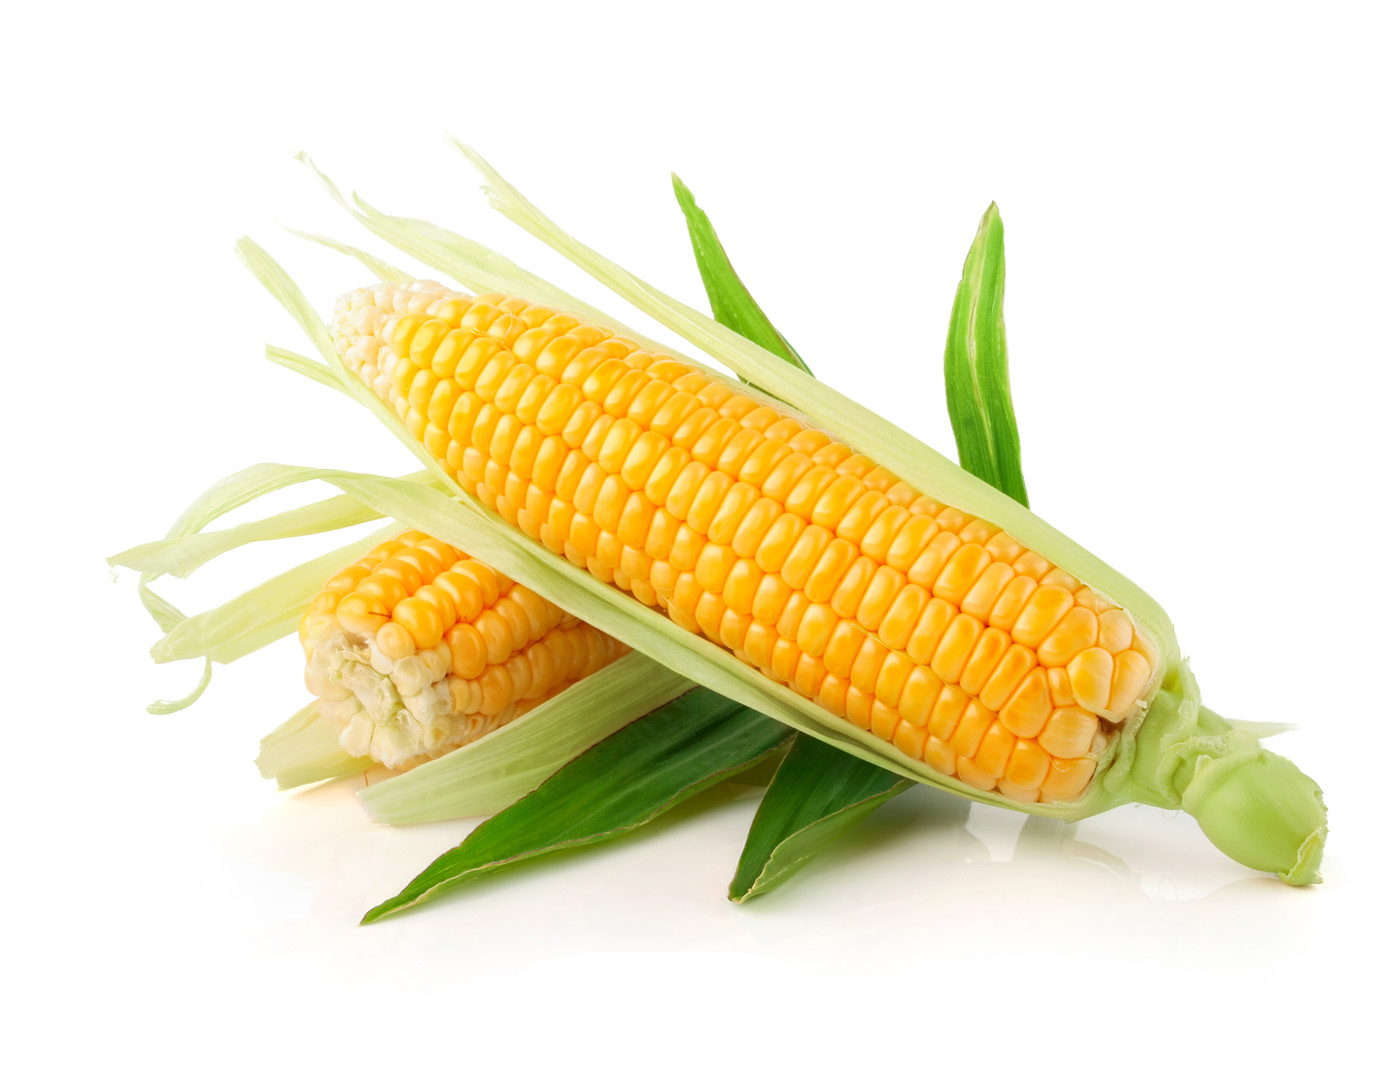
\includegraphics[width=0.5\textwidth]{cob}
	\caption{Pictorial Representation of Full-grown Natively-produced Corn~\cite{Jean2003}}
	\label{fig:corn}
\end{figure}

\section{Corn Production}

	Corn production consist of 10 growth stages. Initially, it starts from planting to seed emergence in Growth Stage 0. Then stages 1 to 4 counts the number of leaves that are completely unfolded. Succeeding stages describe the appearance of the corn cob and the grain mass changes. The 9th stage describe the physiological maturity. Lastly, kernels are dried in growth stage 10 and the corn is now fully grown.

	Production of Corn requires specific environmental requirements for it to grow. This crop is considered a warm weather crop; hence, it is grown in areas with temperature more than 19 degrees Celsius. Germination of the seeds require a minimum of 10 degrees Celsius temperature but an increase in the soil temperature up to a certain degree would allow a faster growth for Maize. 32 degrees Celsius is the approximate critical temperature that could dangerously affect the yielding of the corn. Another environmental factor required is water. Each crop is estimated to have used 250 liters of water in the absence of moisture stress at maturity. Last on the environmental requirement is the soil; it is the most crucial factor that could greatly affect the production of corn. Suitable soil for corn is loam soil -- it must have morphological properties, good internal drainage, and optimal moisture regime.~\cite{Jean2003} 

\section{Agricultural Technology}

Agricultural Technologies are basically equipment used and developed for agricultural purposes. Tools such as Plough, Yoke, Mallot, Sickle, etc. are considered Traditional tools. More advanced tools include tractor, chisel plough, hydrophonics, sprinkler system and many others.

	Agricultural Technologies allowed considerable progression in crop production. Many public and private sector organizations develop these with the aim to address the various biotic and abiotic constraints. With the advancement in tools, America is able to implement Modern Agriculture, a wide type of production. It is an agriculture system wherein farmers use higher end technology and information to control most components of the system. In contrast with the traditional farmers who personally work with resources at hand, modern farmers are dependent on linkages--access to resources, technology, management, and many others. Productivity has increased as machines and computers have eliminated laborious parts of the job. ~\cite{Motes}
	
\section{Agricultural Robots}

	Agricultural robots are designed to be implemented on an unstructured environment. Hence, these robots are expected to be dynamic, uncertain, complex, highly variable, and hostile. In order to build an agricultural robot, multiple design principles are taken into consideration. This includes product specification such as speed, system analysis such as the function, concept development such as alternative methods, feasibility, and what not. Figure~\ref{fig:robot} shows the flowchart  of the implementation of concepts on an agricultural robot.~\cite{Edan}

\begin{figure}[!htbp]
	\centering
		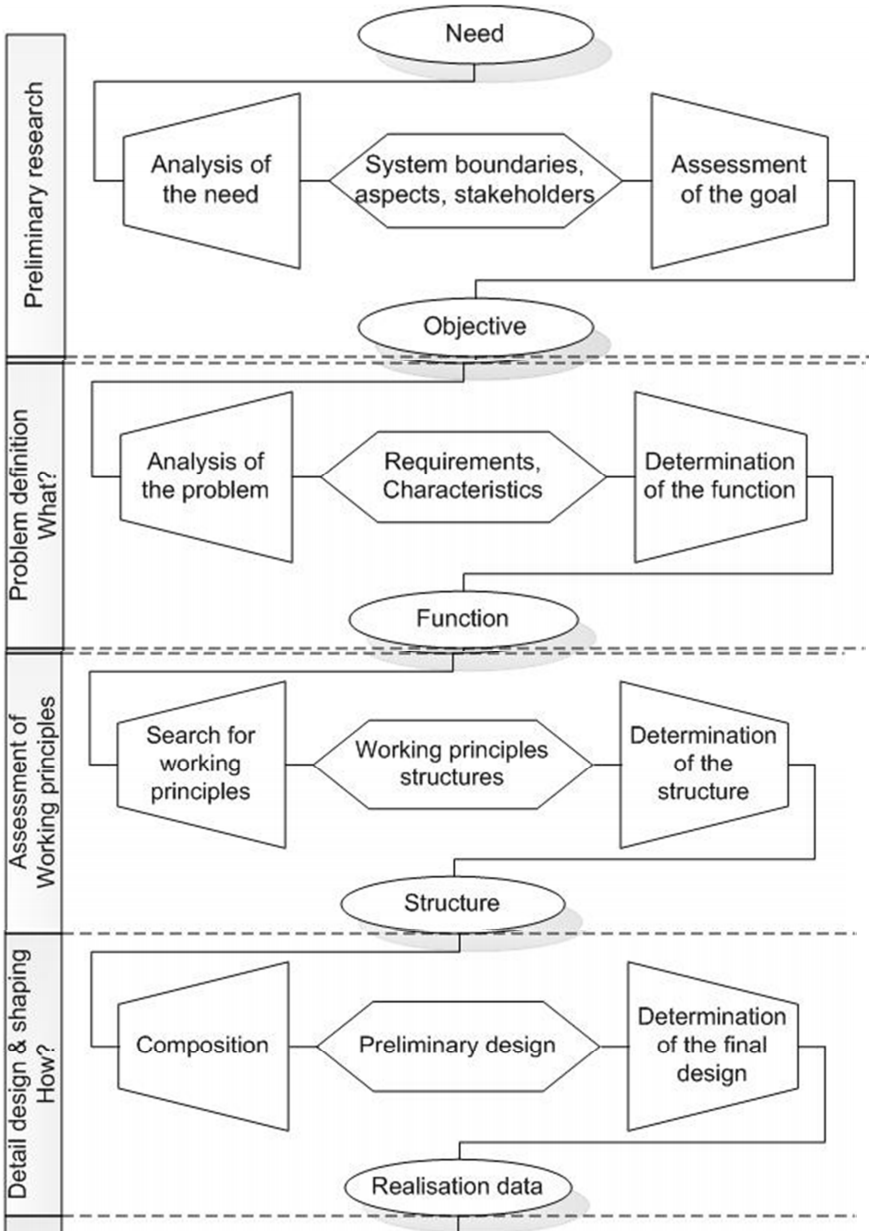
\includegraphics[width=2.5 in]{robot}
	\caption{Flowchart of Agricultural Robot Design~\cite{Edan}}
	\label{fig:robot}
\end{figure}

\section{Philippine Agriculture}

The Philippines is rich in agricultural lands, where about one-third of the land area of 30 million hectares is classified as is. In the year 2013, about 30\% of the Filipino workforce has been employed in this sector.~\cite{WorldBank}. The major contributors to agriculture's gross value is known to be food crops, specifically rice and corn. The croplands of the Philippines are presently under sever environmental stress such as decresing man-land ratio has led the landless to occupy and cultivate ecologically unstable marginal lands. Other problems have emerged as well in the sector of agriculture. Urgency for food security, employment generation to meet the 10-point agenda of the government, and greater global competitiveness trigger the major concerns of the Philippine agricultural sector. In order to respond to this urgent needs of an increasing population while poverty also increases, the Philippine agricultural sector in general has embraced the credo of conventional agricultural practices.~\cite{Briones}
